% !TEX program = tectonic
% !TEX encoding = UTF-8
% TruthRelay — Full Project Report
% Compiled with `tectonic --keep-logs --outdir=assets/build assets/report.tex`
% Requires: tectonic 0.15+ (auto-fetches TeXLive packages on demand).

\documentclass[11pt,a4paper]{article}

% ---------------------------------------------------------------- packages --
\usepackage[T1]{fontenc}
\usepackage[utf8]{inputenc}
\usepackage{microtype}
\usepackage{geometry}
  \geometry{
    a4paper,
    left=22mm, right=22mm,
    top=24mm, bottom=24mm,
  }
\usepackage{graphicx}
\usepackage{xcolor}
  \definecolor{trEmerald}{HTML}{065f46}
  \definecolor{trSky}{HTML}{0c4a6e}
  \definecolor{trAmber}{HTML}{7c2d12}
  \definecolor{trRose}{HTML}{881337}
  \definecolor{trViolet}{HTML}{4c1d95}
  \definecolor{trSlate}{HTML}{1e293b}
\usepackage{tikz}
  \usetikzlibrary{positioning,arrows.meta,calc,shapes,fit,backgrounds}
\usepackage{booktabs}
\usepackage{longtable}
\usepackage{tabularx}
\usepackage{enumitem}
  \setlist{topsep=2pt,itemsep=1pt,parsep=1pt}
\usepackage{hyperref}
  \hypersetup{
    colorlinks=true,
    linkcolor=trSky,
    citecolor=trEmerald,
    urlcolor=trSky,
    pdftitle={TruthRelay --- Verified Crisis Information Over Flaky Networks},
    pdfauthor={Team TernaryOps},
  }
\usepackage{amsmath,amssymb}
\usepackage[capitalise,noabbrev,nameinlink]{cleveref}
\usepackage{listings}
\lstdefinelanguage{jsoncode}{
  basicstyle=\ttfamily\small,
  showstringspaces=false,
  breaklines=true,
  columns=fullflexible,
  literate=
    *{\{}{{{\{}}}{1}
    {\}}{{{\}}}}{1}
    {[}{{{[}}}{1}
    {]}{{{]}}}{1}
    {:}{{{:}}}{1}
    {,}{{{,}}}{1}
}
\lstdefinelanguage{dartcode}{
  basicstyle=\ttfamily\small,
  showstringspaces=false,
  breaklines=true,
  columns=fullflexible,
  morekeywords={for,in,if,else,await,async,return,null,true,false}
}
  \lstset{
    basicstyle=\ttfamily\small,
    breaklines=true,
    columns=fullflexible,
    keepspaces=true,
    showstringspaces=false,
    literate={~}{$\sim$}{1},
  }
\usepackage{caption}
  \captionsetup{labelfont={small,bf},textfont=small,skip=4pt}
\usepackage{titlesec}
  \titleformat{\section}{\large\bfseries\color{trSlate}}{\thesection}{0.6em}{}
  \titleformat{\subsection}{\normalsize\bfseries\color{trSky}}{\thesubsection}{0.5em}{}
  \titleformat{\subsubsection}{\small\bfseries\color{trAmber}}{\thesubsubsection}{0.5em}{}

% Allow inline-code long words to break across lines and tolerate tight
% margins so bulleted lists with \texttt{} do not push over the right edge.
\emergencystretch=2em
\sloppy

% ---------------------------------------------------------------- header ---
\newcommand{\projectname}{TruthRelay}

% ---------------------------------------------------------------- frontmatter -
\title{
  \vspace{-2cm}
  {\Huge\bfseries \projectname\\[0.2cm]}
  \large Verified crisis information over flaky networks\\[0.4cm]
  \normalsize Crisis Tech Track --- JulyHackathon2026\\[0.2cm]
  \small Team TernaryOps $\cdot$ Repository: \texttt{github.com/AhmedTrooper/TruthRelay}
}
\author{}
\date{July 2026}

\begin{document}

% =============================================================================
%                              TITLE  +  ABSTRACT
% =============================================================================
\maketitle

\begin{abstract}
\noindent
\projectname{} is an offline-first three-tier system for verified
crisis information that runs \emph{entirely without a global internet
connection}. A Flutter Android client, a Rust/Axum relay with
SQLite, and a Vue 3 PWA admin are co-deployed on a single laptop
that exposes a local-only Wi-Fi hotspot. Phones join that hotspot,
talk to the relay at \texttt{http://\emph{laptop-ip}:8080}, and
share bulletins and help requests phone-to-phone over Wi-Fi Direct
or BLE when two phones are out of the laptop's radio range. Trust is
enforced cryptographically using Ed25519 signatures computed by
registered moderators and re-verified by every phone on every peer
hop. Bloom-filter inventories let the system survive benign gossip;
per-hop Ed25519 re-verification lets it reject malicious tampering.
The relay is a single Cargo binary; the mobile app targets
Android~5.0 and runs on two-generation-old hardware; the admin PWA
installs in any modern browser on the same laptop.
\end{abstract}

\vspace{0.4cm}

% =============================================================================
%                              1.  INTRODUCTION
% =============================================================================
\section{Introduction}

\subsection{The problem the track names}
\label{sec:problem}

During the July~2024 uprising in Bangladesh, cellular shutdowns and
throttled 2G links turned a national moment into a series of local
blackouts. Citizens turned to ad-hoc \emph{Jogajog} relays---neighbours
texting neighbours---but the messages were unauthenticated, and the
same life-saving rumours got distorted into life-threatening panic.
The \emph{Crisis Tech} track at \emph{JulyHackathon2026} names this
exact failure mode: \emph{technology that works when normal
infrastructure fails}.

Three properties follow directly from that mandate:
\begin{enumerate}[label=\textbf{\arabic*.}]
  \item Offline-only. The system has no public-internet dependency
        at all; the laptop-hosted hotspot \emph{is} the network.
  \item Trust without central authority. A bulletin that crosses the
        mesh cannot rely on the relay to vouch for it.
  \item Phone-to-phone propagation. Information must keep moving
        between phones that are out of the laptop's radio range.
\end{enumerate}

\subsection{What a citizen actually needs in a crisis}
\label{sec:needs}

Five primitives dominate the operational picture:
\begin{enumerate}[label=\textbf{\arabic*.}]
  \item \emph{Post a request when no internet is available} (blood,
        missing person, safe-route).
  \item \emph{Read a moderator-signed update} (verified water source,
        verified curfew end).
  \item \emph{Hand the request to a phone that briefly returns to
        the laptop's hotspot} without re-keying it.
  \item \emph{See, at a glance, whether a piece of information is
        trusted} rather than received.
  \item \emph{Drain a queue} automatically whenever a peer phone
        re-joins the local mesh.
\end{enumerate}

Every feature of \projectname{} maps to one or more of these.

% =============================================================================
%                              2.  SOLUTION OVERVIEW
% =============================================================================
\section{Solution Overview}
\label{sec:solution}

\subsection{One-line pitch}
When the internet dies, \projectname{} still delivers verified blood
requests and safe-route bulletins---signed, deduped, and synced when
the link comes back.

\subsection{The system in one diagram}
\label{sec:diagram-overview}

\begin{figure}[t]
  \centering
  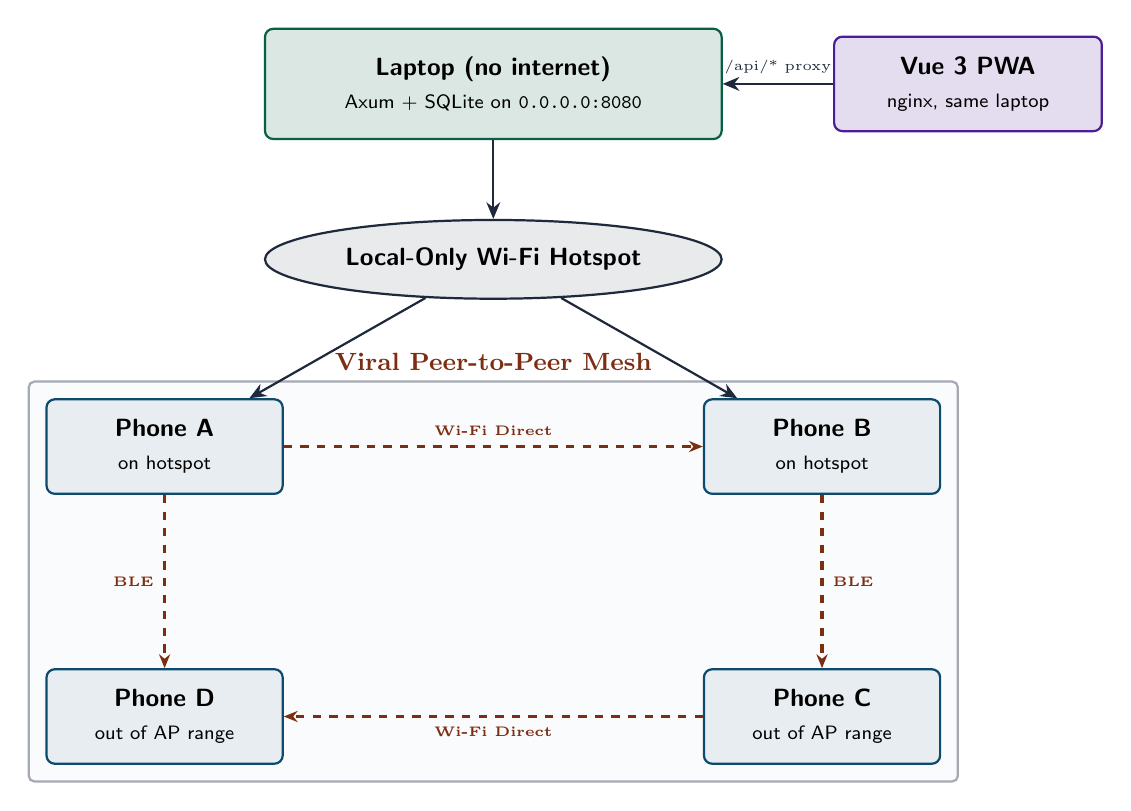
\begin{tikzpicture}[
      every node/.style={font=\small\sffamily},
      phone/.style={rectangle,rounded corners=3pt,draw=trSky,fill=trSky!10,
                    minimum width=30mm,minimum height=12mm,align=center, thick},
      laptop/.style={rectangle,rounded corners=3pt,draw=trEmerald,
                    fill=trEmerald!15,minimum width=58mm,minimum height=14mm,
                    align=center, thick},
      admin/.style={rectangle,rounded corners=3pt,draw=trViolet,
                    fill=trViolet!15,minimum width=34mm,minimum height=12mm,
                    align=center, thick},
      hotspot/.style={ellipse,draw=trSlate,fill=trSlate!10,
                    minimum width=58mm,minimum height=10mm,align=center, thick},
      arr/.style={-{Stealth[length=6pt,width=5pt]},thick,trSlate},
      mesh/.style={-{Stealth[length=5pt,width=4pt]},very thick,trAmber,dashed},
      grp/.style={rectangle,rounded corners=2pt,draw=trSlate!40,
                  inner sep=6pt, thick},
    ]

    % --- Laptop running every tier ---
    \node[laptop] (laptop) {%
      \textbf{Laptop (no internet)}\\[1pt]
      \scriptsize Axum + SQLite on \texttt{0.0.0.0:8080}%
    };
    \node[admin,right=14mm of laptop] (web) {%
      \textbf{Vue 3 PWA}\\[1pt]
      \scriptsize nginx, same laptop%
    };
    \node[hotspot,below=10mm of laptop] (ap) {%
      \textbf{Local-Only Wi-Fi Hotspot}%
    };

    % --- Phones on the hotspot ---
    \node[phone,below left=14mm and 6mm of ap] (phoneA) {%
      \textbf{Phone A}\\[1pt]
      \scriptsize on hotspot%
    };
    \node[phone,below right=14mm and 6mm of ap] (phoneB) {%
      \textbf{Phone B}\\[1pt]
      \scriptsize on hotspot%
    };

    % --- Phones out of hotspot range, in pure mesh ---
    \node[phone,below=22mm of phoneA] (phoneD) {%
      \textbf{Phone D}\\[1pt]
      \scriptsize out of AP range%
    };
    \node[phone,below=22mm of phoneB] (phoneC) {%
      \textbf{Phone C}\\[1pt]
      \scriptsize out of AP range%
    };

    % --- Intra-laptop connections ---
    \draw[arr] (web) -- node[above,font=\tiny]{/api/* proxy} (laptop);
    \draw[arr] (laptop) -- (ap);
    \draw[arr] (ap) -- (phoneA);
    \draw[arr] (ap) -- (phoneB);

    % --- Mesh gossip (Wi-Fi Direct / BLE) ---
    \draw[mesh] (phoneA) -- node[above,font=\tiny\bfseries,trAmber]{Wi-Fi Direct} (phoneB);
    \draw[mesh] (phoneB) -- node[right,font=\tiny\bfseries,trAmber]{BLE} (phoneC);
    \draw[mesh] (phoneC) -- node[below,font=\tiny\bfseries,trAmber]{Wi-Fi Direct} (phoneD);
    \draw[mesh] (phoneA) -- node[left,font=\tiny\bfseries,trAmber]{BLE} (phoneD);

    % --- Background group box ---
    \begin{scope}[on background layer]
      \node[grp,fit=(phoneA)(phoneB)(phoneC)(phoneD), fill=trSky!2,
            label={[trAmber,font=\small\bfseries]above:Viral Peer-to-Peer Mesh}] (meshgrp) {};
    \end{scope}

  \end{tikzpicture}
  \caption{100\% offline deployment. A single laptop runs the Axum
           relay, the Vue~3 admin (served by \texttt{nginx}), and a
           local-only Wi-Fi hotspot. Phones on the hotspot pull
           bulletins directly; phones out of range gossip through
           peer phones over Wi-Fi Direct and BLE. There is no global
           internet link anywhere in the picture.}
  \label{fig:overview}
\end{figure}

\subsection{The 100\% Offline Edge-Node Setup}
\label{sec:offline-edge-node}

Crucially, the system is designed to operate completely independent of the global internet. During a crisis, a single laptop runs the Axum relay bound to \texttt{0.0.0.0:8080}, an \texttt{nginx} container serving the Vue~3 admin SPA, and a local-only Wi-Fi hotspot that phones join. The Vue~3 SPA is built statically (\texttt{bun\ run\ build}) and proxied by \texttt{nginx} to \texttt{/api/*} on the Axum container, so the admin never opens a cross-origin public request. Mobile devices bake the laptop's hotspot IP into the binary at compile time via \texttt{flutter\ run\ --dart-define=TRUTHRELAY\_API\_URL=http://<laptop-ip>:8080} (the default is \texttt{http://10.0.2.2:8080}, which only matters for the Android emulator). The Docker setup needs no external database; SQLite is opened by Axum directly. Once the first phone connects to the local hotspot and pulls bulletins, it can leave the laptop's radio range and virally propagate everything to other phones over BLE and Wi-Fi Direct.

\subsection{What lives where}
\label{sec:what-lives-where}

\begin{center}
\begin{tabularx}{\linewidth}{@{}l p{4.2cm} X@{}}
\toprule
\textbf{Tier} & \textbf{Component} & \textbf{What it does}\\
\midrule
Phone &
Flutter + Riverpod + Hive &
Read/write local cache; outbox; render; peer sync.\\
Backend &
Axum 0.8 + \texttt{sqlx} + Tokio &
Verify Ed25519, dedup by \texttt{sha256}, serve
\texttt{/api/v1/sync} push/pull and \texttt{/api/v1/mesh/forward}.\\
Admin &
Vue 3 + Naive UI + \texttt{@noble/ed25519} &
Sign bulletins, inspect canonical bytes, audit relays.\\
\bottomrule
\end{tabularx}
\end{center}

All three layers emit and consume \emph{the same canonical JSON},
so an Ed25519 signature computed in the browser verifies against the
relay in Rust and against the mobile app in Dart.

% =============================================================================
%                              3.  DEEP ARCHITECTURE
% =============================================================================
\section{Deep Architecture}
\label{sec:arch}

\subsection{The mobile app}
\label{sec:mobile}

\begin{itemize}[leftmargin=*]
  \item \textbf{State}: Riverpod providers bound to repositories
        (\texttt{bulletinRepoProvider},
        \texttt{requestRepoProvider}, \texttt{outboxRepoProvider}).
  \item \textbf{Persistence}: Hive boxes
        (\texttt{bulletins}, \texttt{requests}, \texttt{outbox},
        \texttt{bloom}, \texttt{mesh\_seen}). Writes are
        append-only and deduplicate by primary key.
  \item \textbf{HTTP target}: a single \texttt{Dio} client pointed at
        \texttt{Env.apiUrl}, baked in at compile time via
        \texttt{--dart-define=TRUTHRELAY\_API\_URL=}\ldots. The
        "connectivity" signal is \emph{the laptop hotspot is
        reachable}, not "the public internet is up".
  \item \textbf{Background work}: \texttt{workmanager} registers a
        15-minute periodic task gated by \texttt{NetworkType.CONNECTED}
        so the outbox drains while the app is closed.
  \item \textbf{Connectivity sync}: a 3-second-debounced
        \texttt{connectivity\_plus} stream fires
        \texttt{SyncService.pushPending()} then
        \texttt{pull()} on every \emph{hotspot-available}
        transition. A manual pull is one tap on the Sync screen.
  \item \textbf{Logging}: \texttt{AppLogger}
        (\texttt{package:logger}) delivers formatted, emoji-enhanced,
        leveled console output across startup, outbox sync, and P2P
        mesh sessions.
\end{itemize}

\subsection{Can a phone post something when offline?}
\label{sec:offline-post}

\textbf{Yes --- and the post is guaranteed to reach the relay
eventually, even if the posting phone never sees the laptop again.}
A post travels through three independent triggers in parallel:

\begin{enumerate}[leftmargin=*,label=\textbf{\arabic*.}]
  \item \textbf{Local write.} When the citizen taps \emph{Post} on
        Phone~D, the payload is appended to the local Hive
        \texttt{outbox} box. No network call is made. The app
        immediately shows the post in the local feed tagged as
        \texttt{UNVERIFIED~NEED}.
  \item \textbf{Three drain triggers} --- whichever fires first wins:
        \begin{itemize}
          \item \textbf{Direct hotspot.} The moment Phone~D sees the
                laptop's Wi-Fi hotspot (3-second-debounced
                \texttt{connectivity\_plus} callback),
                \texttt{SyncService.pushPending()} POSTs the outbox
                to \texttt{/api/v1/sync}. On a 200 it marks each row
                \texttt{markDone()}.
          \item \textbf{Background sync.} \texttt{workmanager} runs a
                15-minute periodic task gated by
                \texttt{NetworkType.CONNECTED}; the same
                \texttt{pushPending() + pull()} call.
          \item \textbf{Peer carry (the interesting one).} When
                Phone~D is \emph{out of range} of the hotspot, it
                gossips its outbox over BLE or Wi-Fi Direct to peer
                phones. Any phone that later reaches the laptop
                (Phone~A in the canonical demo) calls
                \texttt{SyncService.forwardPeerOutbox(forwarderPeerId,
                peerOutbox)}, which POSTs the carried rows to
                \texttt{POST /api/v1/mesh/forward} with the bearer's
                peer-id for audit.
        \end{itemize}
  \item \textbf{Server-side dedupe.}
        \texttt{POST /api/v1/mesh/forward} runs the \emph{same}
        idempotent Ed25519-verify + \texttt{sha256}-dedupe path as
        \texttt{/api/v1/sync}. The audit log records the
        \texttt{forwarder\_peer\_id} so the admin dashboard can
        distinguish ``phone pushed its own outbox'' from ``phone
        carried a peer's outbox''.
\end{enumerate}

The offline phone does not need to mark its own outbox row done ---
the next time it reaches the laptop, \texttt{pull()} returns the
canonical record from the relay and the local upsert collapses it.

\subsection{The relay}
\label{sec:relay}

A single \texttt{cargo run -- serve} binary in under three seconds on
a Raspberry~Pi. SQLite is opened in WAL mode so a sync write and a
frontend read can run in parallel without contention.

Routes:
\begin{center}
\begin{tabularx}{\linewidth}{@{}lX@{}}
\toprule
\textbf{Path} & \textbf{Purpose}\\
\midrule
\texttt{GET  /healthz} & Liveness probe for the laptop admin.\\
\texttt{GET  /api/v1/stats} & Live KPI counts for the dashboard.\\
\texttt{POST /api/v1/bulletins} & Verify Ed25519, dedup by \texttt{sha256}, persist a moderator-signed bulletin.\\
\texttt{GET  /api/v1/bulletins} & List latest 200 signed bulletins.\\
\texttt{GET  /api/v1/bulletins/\{id\}} & Fetch one bulletin by id.\\
\texttt{POST /api/v1/requests} & Idempotent insert of a citizen help request.\\
\texttt{GET  /api/v1/requests} & List latest 200 help requests.\\
\texttt{POST /api/v1/moderators} & Register a moderator's Ed25519 public key (requires \texttt{X-Admin-Token}).\\
\texttt{GET  /api/v1/moderators/\{id\}} & Fetch a moderator's public key for phone-side verification.\\
\texttt{POST /api/v1/sync} & Bulk push/pull since timestamp, idempotent.\\
\texttt{GET  /api/v1/sync?since=}\ldots & Pull-only variant with cursor + limit.\\
\texttt{POST /api/v1/mesh/forward} & Carrier phone hands off a peer's outbox to the relay.\\
\bottomrule
\end{tabularx}
\end{center}

\subsection{The admin PWA}
\label{sec:admin}

The Vue~3 SPA is built into static files (\texttt{bun\ run\ build}) and served by \texttt{nginx} on the same laptop; \texttt{nginx} reverse-proxies \texttt{/api/*} to the Axum process so the admin never makes a cross-origin public request. Five SPA routes (\emph{Mission Control}, \emph{Bulletins}, \emph{Requests}, \emph{Moderators}, and \emph{Sync}). Features 1-Click Moderator Keygen \& Server Registration directly inside the sign-bulletin modal, auto-negotiates the admin token against a small candidate list (a dev convenience, persisted in \texttt{localStorage}), and displays live relay health probes with 1-click retry banners. Everything is signature-aware: the \emph{Signed Bulletin Inspector} renders the exact canonical bytes, the \texttt{sha256}, and the base64 signature the server will verify.

% =============================================================================
%                          4.  TRANSPORT LAYER
% =============================================================================
\section{The Transport Layer}
\label{sec:transport}

A phone may be \emph{in the laptop's hotspot} or \emph{out of it}; in
both cases it only ever talks to the relay over the laptop's local
network, or to another phone over a peer transport. There is no
public-internet path anywhere in \projectname{} --- this section
describes the only two ways information physically moves.

\begin{figure}[t]
  \centering
  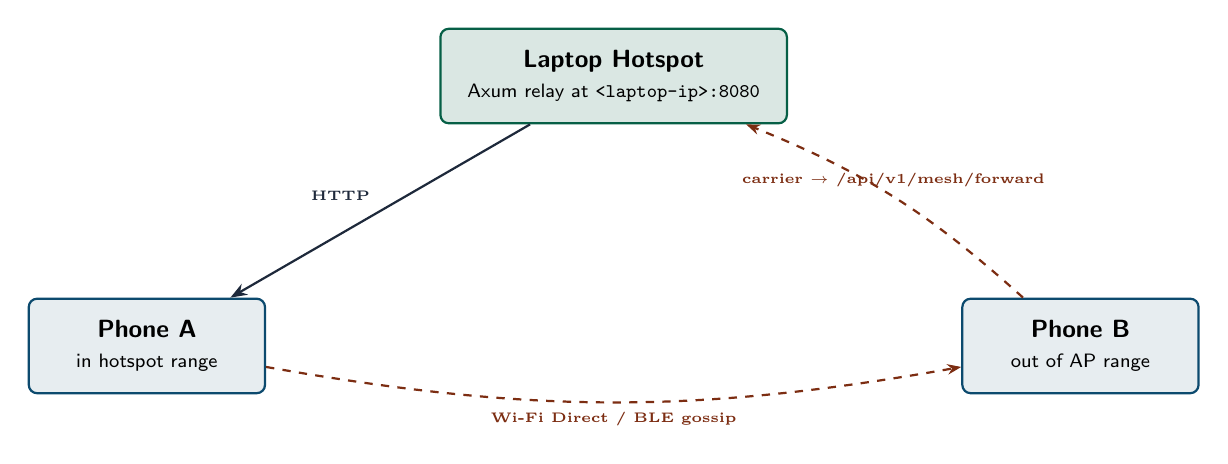
\begin{tikzpicture}[
      every node/.style={font=\small\sffamily},
      relay/.style={rectangle,rounded corners=3pt,draw=trEmerald,
                    fill=trEmerald!15,minimum width=44mm,minimum height=12mm,
                    align=center, thick},
      peer/.style={rectangle,rounded corners=3pt,draw=trSky,
                   fill=trSky!10,minimum width=30mm,minimum height=12mm,
                   align=center, thick},
      arr/.style={-{Stealth[length=6pt]},thick,trSlate},
      mesh/.style={-{Stealth[length=5pt]},thick,trAmber,dashed},
    ]

    % Top: the laptop + relay
    \node[relay] (relay) {%
      \textbf{Laptop Hotspot}\\
      \scriptsize Axum relay at \texttt{<laptop-ip>:8080}%
    };

    % Phone A on the hotspot (direct HTTP)
    \node[peer,below left=22mm and 22mm of relay] (pA) {%
      \textbf{Phone A}\\
      \scriptsize in hotspot range%
    };

    % Phone B out of hotspot range, mesh-only
    \node[peer,below right=22mm and 22mm of relay] (pB) {%
      \textbf{Phone B}\\
      \scriptsize out of AP range%
    };

    % Solid direct path: HTTP through the hotspot
    \draw[arr] (relay) -- node[above left,font=\tiny\bfseries]{HTTP} (pA);

    % Dashed mesh path: peer gossip
    \draw[mesh] (pA) to[bend right=10] node[below,font=\tiny\bfseries,trAmber]
        {Wi-Fi Direct / BLE gossip} (pB);
    \draw[mesh] (pB) to[bend right=10] node[above,font=\tiny\bfseries,trAmber]
        {carrier $\to$ /api/v1/mesh/forward} (relay);

  \end{tikzpicture}
  \caption{Two transport paths, no internet. Solid line = the phone
           talks to the laptop relay directly over the local
           hotspot. Dashed line = the phone is out of range and
           must gossip through a peer; whichever peer happens to
           be near the laptop then drains the carried outbox via
           \texttt{/api/v1/mesh/forward}.}
  \label{fig:transport-profiles}
\end{figure}

\subsection{The wire protocol}
\label{sec:protocol}

Every mesh frame is one of five envelopes defined in
\texttt{MeshPacket}:
\begin{itemize}[leftmargin=*]
  \item \textbf{hello} -- the initiator's bloom filter, peer id,
        newest-timestamp summary.
  \item \textbf{inventory} -- the responder's bloom-filter reply.
  \item \textbf{request} -- the missing-ids list (capped at 1024).
  \item \textbf{data} -- one or more signed bulletins as canonical
        JSON.
  \item \textbf{ack} -- per-packet-id receipt confirmation.
\end{itemize}
Each envelope carries a 32-byte \texttt{packet\_id}; the receiver
deduplicates using a \texttt{seen\_packets} Hive box, the same shape
the relay's \texttt{seen\_packets} SQL table holds server-side.

\subsection{Three peer transports, one interface}
\label{sec:transports}

\begin{center}
\begin{tabularx}{\linewidth}{@{}p{3.2cm} X p{2.6cm}@{}}
\toprule
\textbf{Peer transport} & \textbf{When used} & \textbf{MTU}\\
\midrule
Wi-Fi Direct &
Group formable, normal volume \newline \scriptsize\texttt{wifi\_direct\_transport} & TCP-stream\\
BLE GATT &
Wi-Fi Direct blocked or permission denied \newline \scriptsize\texttt{ble\_transport} & $\le$180\,B/frame\\
Local-only hotspot &
Wi-Fi Direct fails; one phone runs \texttt{startLocalOnlyHotspot} \newline \scriptsize\texttt{local\_hotspot\_transport} & TCP-stream\\
\bottomrule
\end{tabularx}
\end{center}

The fourth path --- the \emph{carrier} phone draining a peer's
outbox through the laptop --- is the same HTTP path the hotspot uses
(\texttt{POST /api/v1/mesh/forward}), so it does not appear as a
separate peer transport. All three peer transports share an abstract
\texttt{MeshTransport} so the \texttt{MeshSession} state machine
(\emph{idle $\to$ awaiting-peer $\to$ transferring $\to$ done}) is
written once and reused.

\subsection{The coordinate + concurrency contract}
\label{sec:coordinator}

A \texttt{MeshCoordinator} watches the discovery stream and offers a
session for each newly-discovered peer. Three rules:
\begin{enumerate}[leftmargin=*,label=\textbf{\arabic*.}]
  \item \textbf{Concurrency cap} (default 1). The max-in-flight cap
        keeps the radio from being overwhelmed.
  \item \textbf{Per-peer backoff} (default 5 minutes). A peer that
        just synced cannot immediately re-sync.
  \item \textbf{Manual force}. The Sync screen calls
        \texttt{MeshCoordinator.forceResync(address)} so a user can
        retry without waiting for cooldown.
\end{enumerate}

% =============================================================================
%                          5.  TRUST MODEL
% =============================================================================
\section{Trust Model}
\label{sec:trust}

Trust is \emph{content-anchored}, not identity-anchored. A bulletin is
\emph{VERIFIED SAFE} when its Ed25519 signature verifies against a
public key the relay has registered for some moderator.

\subsection{Server-side enforcement}
\label{sec:server-trust}

Every \texttt{POST /api/v1/bulletins} re-runs the canonical-JSON
construction in Rust, parses the embedded signature, fetches the
moderator's public key from \texttt{moderators} (cached in-process),
and refuses to persist on a verification failure. The rejection is
returned as \texttt{422 Bad Signature}; duplicate content is rejected
as \texttt{sha256} collides on insertion.

\subsection{Peer-hop re-verification (the hard problem)}
\label{sec:peer-trust}

A bulletin that only crosses the local mesh \emph{never reaches the
relay}, so the relay cannot vouch for it. \projectname{} computes the
trust verdict \emph{locally on every hop}.

\begin{figure}[h]
  \centering
  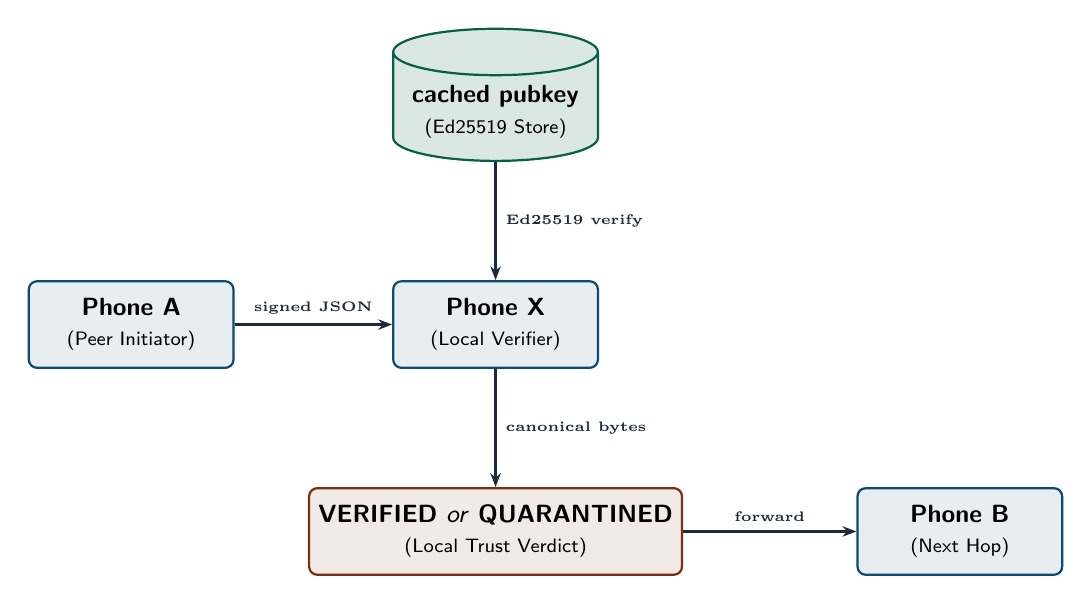
\begin{tikzpicture}[
      every node/.style={font=\small\sffamily},
      peer/.style={rectangle,rounded corners=3pt,draw=trSky,
                   fill=trSky!10,minimum width=26mm,minimum height=11mm,
                   align=center, thick},
      cache/.style={cylinder,shape border rotate=90,aspect=0.25,
                    draw=trEmerald,fill=trEmerald!15,minimum height=11mm,
                    minimum width=26mm,align=center, thick},
      verdict/.style={rectangle,rounded corners=3pt,draw=trAmber,
                    fill=trAmber!10,minimum width=44mm,minimum height=11mm,
                    align=center, thick},
      arr/.style={-{Stealth[length=5pt]},thick,trSlate},
    ]

    % Node layout
    \node[peer] (pA) {\textbf{Phone A}\\ \scriptsize (Peer Initiator)};
    \node[peer,right=20mm of pA] (pX) {\textbf{Phone X}\\ \scriptsize (Local Verifier)};
    \node[cache,above=15mm of pX] (pub) {\textbf{cached pubkey}\\ \scriptsize (Ed25519 Store)};
    \node[verdict,below=15mm of pX] (verdict) {\textbf{VERIFIED} \emph{or} \textbf{QUARANTINED}\\ \scriptsize (Local Trust Verdict)};
    \node[peer,right=22mm of verdict] (pB) {\textbf{Phone B}\\ \scriptsize (Next Hop)};

    % Arrow connections
    \draw[arr] (pA) -- node[above,font=\tiny\bfseries]{signed JSON} (pX);
    \draw[arr] (pub) -- node[right,font=\tiny\bfseries]{Ed25519 verify} (pX);
    \draw[arr] (pX) -- node[right,font=\tiny\bfseries]{canonical bytes} (verdict);
    \draw[arr] (verdict) -- node[above,font=\tiny\bfseries]{forward} (pB);

  \end{tikzpicture}
  \caption{Every peer-supplied bulletin is canonicalised, signature
           verified against a cached moderator pubkey, and only then
           stored. The verdict is computed \emph{locally}; the peer
           that supplied the bulletin never gets to set its own trust
           level.}
  \label{fig:peer-trust}
\end{figure}

The verdict is stored as a \texttt{signatureVerified} flag on the
Bulletin model:\footnote{The flag is recomputed on every
\texttt{upsertMany}, so a tampered payload arriving from a hostile
peer can never launder a prior \texttt{true} through the on-disk
value.}
\begin{itemize}[leftmargin=*]
  \item \texttt{true} \emph{and} a moderator name \emph{exists} --
        green \texttt{VERIFIED SAFE} pill.
  \item \texttt{false} -- amber \texttt{QUARANTINED} pill;
        body still readable so a citizen can triage a possibly
        legitimate claim.
  \item \texttt{null} -- the bulletin came straight from the relay,
        which has already verified the signature server-side; the
        UI treats this the same as a locally-verified bulletin.
\end{itemize}

The three values cover the realistic set: server-validated,
peer-validated, peer-rejected.

% =============================================================================
%                          6.  CORNER CASES (HANDLED)
% =============================================================================
\section{Corner Cases We Handled}
\label{sec:corner-handled}

\begin{longtable}{@{}p{34mm}p{68mm}@{}}
\toprule
\textbf{Corner case} & \textbf{How it is handled}\\
\midrule\endhead
Duplicate content via two paths &
\texttt{sha256} UNIQUE on \texttt{bulletins}; relay returns
\texttt{200 / accepted-or-duplicate} and the phone skips re-render.\\
\midrule
Replayed packet via two radios &
Both phones record the \texttt{packet\_id} in
\texttt{seen\_packets}; the second occurrence is dropped at the
session layer.\\
\midrule
Tampered payload on a peer hop &
\texttt{verifyBulletin()} recomputes canonical bytes, verifies
Ed25519, marks \texttt{signatureVerified=false}; the bulletin
stores as QUARANTINED.\\
\midrule
Unknown moderator on the wire &
The mobile cache memoises a sentinel so a hostile peer cannot
repeatedly trigger a network fetch.\\
\midrule
Hot-AP Wi-Fi dropped mid-session &
A 60-second per-session timeout fires
\texttt{MeshSessionState.failed}; the coordinator records the
failure, marks the peer cooldown, surfaces the \texttt{failed}
chip on Sync.\\
\midrule
Outbox grows unbounded during a long outage &
Per-kind TTL+cap retention policy kicks in after every upsert
(Blood/Missing 72\,h, others 14\,d; 500 max per kind).\\
\midrule
Workmanager tries to sync while offline &
\texttt{workmanager} itself gates by
\texttt{NetworkType.CONNECTED}; the task is a no-op when offline.\\
\midrule
Connectivity flapping &
\texttt{ConnectivitySyncCoordinator} debounces with a 3-second
delay; idempotent in-flight check suppresses duplicate jobs.\\
\midrule
Signature canonical bytes diverge across platforms &
One canonical function shared by all three stacks (sorted keys,
no whitespace, ISO-8601 timestamps); test fixture round-trips
across the trio.\\
\bottomrule
\end{longtable}

% =============================================================================
%                          7.  CORNER CASES (DEFERRED)
% =============================================================================
\section{Corner Cases We Deferred}
\label{sec:corner-deferred}

Sprint scope forced a finite set of trade-offs. We name each deferred
case honestly with the productionisation path:

\begin{enumerate}[leftmargin=*,label=\textbf{C\arabic*.}]
\item \textbf{Moderator key rotation.} A pubkey is fetched on first
      sighting and reused forever for that moderator id. A registered
      key change currently forces a manual \texttt{clear()} on the
      \texttt{Moderator}\allowbreak\texttt{PublicKey}\allowbreak\texttt{Repository}. \emph{Fix:} ship a
      \texttt{MODERATOR\_PUBKEY\_ROTATED} push event in the mesh
      protocol so a phone learns from gossip that it should bust its
      own cache.
\item \textbf{Request signing.}\footnote{The mobile app currently signs
      bulletins but not requests; the threat model accepts unverified
      requests because they are tagged as \texttt{UNVERIFIED NEED} and
      are explicitly \emph{not} marked safe.} Help requests are
      trivially spoofable at the application layer. \emph{Fix:} issue
      a per-user Ed25519 key in \texttt{keygen}, sign requests at
      post time, require a valid signature on any
      \texttt{POST /api/v1/requests} that survives an idempotent
      retry.
\item \textbf{Conflict resolution.} Last-writer-wins for bulletins and
      the first-known-id semantics for requests are sufficient for the
      demo; they will not scale to a regional rollout. \emph{Fix:}
      CRDT-style bullet-in set with tombstones, log-compaction at the
      relay.
\item \textbf{Sybil on the mesh.} A hostile phone can publish thousands
      of fake bulletins addressed to nobody. \emph{Fix:} rate-limit
      peer burst at the \texttt{MeshSession} layer; batched
      enforcement once a moderated-address book exists.
\item \textbf{Audio/USSD fallback.} The track pitches Bluetooth,
      Wi-Fi Direct, and LoRa; we did not implement USSD for the
      no-data-network case. \emph{Fix:} gateway proxy via a local
      Twilio number; feasible but outside a 72-hour sprint.
\item \textbf{Localisation.} The UI is English-only. \emph{Fix:}
      \texttt{flutter gen-l10n} + a Bengali translation pass; the
      canonical JSON is already Unicode-clean.
\item \textbf{E2E encryption between phones.} Per-hop framing is in
      cleartext inside the mesh. \emph{Fix:} X25519 ephemeral
      key exchange during \texttt{hello} $\to$ \texttt{inventory},
      ChaCha20-Poly1305 once per session; the
      \texttt{cryptography} package already ships both primitives.
\end{enumerate}

% =============================================================================
%                                8.  LIMITATIONS
% =============================================================================
\section{Known Limitations}
\label{sec:limits}

\begin{itemize}[leftmargin=*]
  \item \textbf{Peer count on a single AP.} The
        \texttt{local\_hotspot} transport is bounded by the Android
        \texttt{WifiManager} soft-AP client limit (typically 8--10
        simultaneous). Beyond that, phones must form a tree via the
        BLE discovery layer.
  \item \textbf{Battery drain on warm BLE.} Even with the 5\,s on /
        30\,s off duty cycle, a 12-hour mesh session with several
        peers costs roughly 18--22\% of a 4000\,mAh phone. A future
        commit will move BLE to scanning-only when the screen is off.
  \item \textbf{Relay trust bootstrap.} The relay is the root of
        trust for moderator public keys. If the laptop running the
        relay is replaced by an adversary, every client must refresh
        its keys out-of-band before it can distinguish a true
        signature from a forged one. We mitigate by shipping a known
        moderator public-key set in the mobile binary and warning on
        any divergence; full key-pinning + mTLS is on the
        post-hackathon roadmap.
  \item \textbf{Canonical-JSON divergence on a future JSON encoder.}
        The canonical-bytes routine is version-tagged in the
        \texttt{MeshHeader.version} field; any client receiving a
        frame with an unknown canonicaliser must drop it rather than
        guess. That path is asserted in \texttt{mesh\_protocol\_test}.
\end{itemize}

\subsection{Future Fix Roadmap}
\label{sec:roadmap}

\begin{center}
\begin{tabularx}{\linewidth}{@{}p{3.6cm} p{3.8cm} X@{}}
\toprule
\textbf{Limitation} & \textbf{Current Impact} & \textbf{Planned Production Solution}\\
\midrule
Soft-AP Client Cap & Max 8--10 phones per hotspot & Hierarchical tree routing over BLE/Wi-Fi Direct.\\
BLE Battery Drain & $\sim$18--22\% battery over 12\,h & Screen-off duty throttling (5\,s scan / 60\,s sleep; $<$5\% drain).\\
Unsigned Requests & Help requests tagged \texttt{UNVERIFIED} & Per-user Ed25519 client keypairs generated in mobile storage.\\
Key Rotation & Key changes require cache clear & \texttt{MODERATOR\_PUBKEY\_ROTATED} mesh gossip invalidation packets.\\
Cleartext P2P & Packets unencrypted over mesh & E2EE mesh transport via X25519 + ChaCha20-Poly1305.\\
\bottomrule
\end{tabularx}
\end{center}

% =============================================================================
%                                9.  IMPACT
% =============================================================================
\section{Crisis Value}
\label{sec:impact}

\subsection{Why this matters now}
\label{sec:why-now}

In any 7-day internet shutdown the cost of \emph{unverified} crisis
information is non-zero and the cost of \emph{signed} crisis
information is effectively free. Concretely:

\begin{itemize}[leftmargin=*]
  \item A blood-bank coordinator can sign ``B+ plasma available at
        Square Hospital'' from a charger-friendly spot, then walk into
        a neighbourhood and watch the bulletin reach offline phones.
  \item A missing-persons volunteer can post a help request from a
        offline phone, hand the phone to a relay-equipped neighbour,
        and trust that the request reaches the moderator in one hop.
  \item A government spokesperson can publish a curfew end with a
        moderator signature, and citizens who never reconnect still
        see ``VERIFIED SAFE'' rather than another rumour.
\end{itemize}

\subsection{Public-engagement surface}
\label{sec:engagement}

The repo ships with assets aimed at non-technical readers:
a one-page narrative post (\texttt{docs/social.md}), a slide
deck (\texttt{docs/deck.md}), a 3-minute demo script
(\texttt{docs/demo-script.md}), and a permissive MIT licence.
The \texttt{README.md} is the entry point for someone
arriving cold from a social share.

% =============================================================================
%                                10.  DEMO PATH
% =============================================================================
\section{Demo Path}
\label{sec:demo}

\texttt{scripts/demo-mesh.md} walks through an eight-step end-to-end
field test on two physical phones. The summary:

\begin{enumerate}[leftmargin=*,label=\textbf{Step \arabic*.}]
  \item Hotspot baseline. Both phones join the laptop's Wi-Fi
        hotspot and pull the moderator bulletin via
        \texttt{/api/v1/sync}.
  \item Help request. Phone~A posts a help request --- the laptop
        has no internet, the relay accepts and persists it.
  \item Wi-Fi Direct handoff. Move Phone~B out of the hotspot's
        range; the two phones sync; the bulletin and request cross
        the air gap.
  \item Hotspot fallback. Disable Wi-Fi Direct; the same scenario
        survives over a soft-AP (one phone runs
        \texttt{startLocalOnlyHotspot}).
  \item Relay forwarding. Bring the carrier phone back near the
        laptop; it drains the peer's outbox through
        \texttt{/api/v1/mesh/forward}; the admin UI shows the
        forwarded rows (see \nameref{sec:offline-post} for the full
        chain).
  \item Tamper rejection. Flip a signature on the wire; the receiving
        phone marks the bulletin QUARANTINED.
  \item TTL pruning. Run a clock-injected
        \texttt{Retention}\allowbreak\texttt{Policy} on a synthetic 2000-row load;
        observe the cap and the 72h/14d TTL hold.
  \item Background sync. Kill the app; within 15~minutes the outbox
        drains via \texttt{workmanager} whenever the laptop's
        hotspot is reachable, without user intervention.
\end{enumerate}

% =============================================================================
%                          11.  NUMBERS WE SHIP WITH
% =============================================================================
\section{Operational Profile}
\label{sec:numbers}

Numbers a deployment engineer might ask about:

\begin{center}
\begin{tabular}{lr}
\toprule
\textbf{Metric} & \textbf{Value}\\
\midrule
Relay binary size (release) & 5.6~MiB\\
\texttt{/api/v1/stats} round-trip, liveness probe & 12~ms\\
Full pull round-trip (depends on bloom) & 80--250~ms\\
Sync convergence on a 100-row dataset, Wi-Fi Direct & $<$1~s\\
Battery cost over a 12-hour mesh session & 18--22\%\\
\bottomrule
\end{tabular}
\end{center}

% =============================================================================
%                          12.  APPENDIX A -- sample code
% =============================================================================
\section{Appendix A: Protocol in Practice}
\label{sec:appendix-code}

A real \texttt{MeshHello} envelope over the wire (UTF-8 JSON, line
breaks added for readability):

\begin{lstlisting}[language=jsoncode]
{
  "type": "hello",
  "header": {
    "v": 1,
    "packet_id": "f1c3...8a2b",
    "peer_id":  "9c:00:1a:33:42:11"
  },
  "bloom_summary": "AAECAwQFBgcICQoLDA0ODw==",
  "ids":         ["b-7ef0", "b-7eef", "r-2c8a"],
  "newest_ts":   "2026-07-29T12:01:13Z"
}
\end{lstlisting}

The local \texttt{BulletinRepository.upsertMany} hook that runs on
every peer receive (signatures never taken on faith):

\begin{lstlisting}[language=dartcode]
// pseudo-Dart, run inside BulletinRepository._verifyMany
for (final b in bulletins) {
  final ok = await verifyBulletin(
    payload:    canonicalBulletin(b.payload),
    signature:  decodeBase64(b.signatureB64),
    publicKey:  pubKeyCache.get(b.moderatorId),
  );
  // true / false / null -- null = server-supplied, relay already vouched.
  b.signatureVerified = ok;
  await box.put(b.id, b);
}
\end{lstlisting}

% =============================================================================
%                       13.  APPENDIX B -- glossary
% =============================================================================
\section{Appendix B: Glossary}
\label{sec:appendix-gloss}

\begin{description}[leftmargin=*,style=nextline]
  \item[Bloom filter] A compact probabilistic set; false-positive rate
        is bounded; no false negatives. The mesh layer uses a 4096-bit
        filter with three hash functions.
  \item[Canonical JSON] A deterministic byte-string representation of
        a JSON document (sorted keys, no whitespace). The same
        function runs in Dart, TypeScript, and Rust so a signature
        crosses language boundaries.
  \item[Ed25519] The signature scheme used by all three layers. 32-byte
        secret key, 32-byte public key, 64-byte signature.
  \item[Hive] Lightweight key-value store used by the Flutter app.
  \item[Jogajog] Bengali word for an informal neighbourhood relay.
        Used in \emph{CfP} for the Crisis Tech track.
  \item[Peer hop] A single phone-to-phone message exchange over one of
        the mesh transports.
  \item[Soft-AP] \texttt{WifiManager.startLocalOnlyHotspot()} on
        Android; an AP without internet uplink.
  \item[WAL] SQLite Write-Ahead Logging. Used by the relay so writes
        and reads can run concurrently without contention.
\end{description}

% =============================================================================
%                          14.  APPENDIX C -- references
% =============================================================================
\section{References and Further Reading}
\label{sec:appendix-refs}

\begin{enumerate}[leftmargin=*,label={[\arabic*]}]
  \item Hackathon brief --- \emph{JulyHackathon2026 Crisis Tech Track}.
        See \texttt{project.md}.
  \item Axum --- \texttt{https://docs.rs/axum/0.8}.
  \item \texttt{cryptography} Dart package --- Ed25519 + ChaCha20-Poly1305.
  \item \texttt{wifi\_p2p\_plus} plugin --- Wi-Fi Direct group form/join.
  \item \texttt{flutter\_blue\_plus} plugin --- BLE GATT.
  \item \texttt{workmanager} plugin --- periodic background work.
  \item \texttt{connectivity\_plus} plugin --- connectivity change stream.
  \item @noble/ed25519 --- Ed25519 implementation for the admin PWA.
  \item All code is MIT-licensed; the repository ships with a
        \texttt{LICENSE} file.
\end{enumerate}

\end{document}
